%% bare_conf.tex
%% V1.3
%% 2007/01/11
%% by Michael Shell
%% See:
%% http://www.michaelshell.org/
%% for current contact information.
%%
%% This is a skeleton file demonstrating the use of IEEEtran.cls
%% (requires IEEEtran.cls version 1.7 or later) with an IEEE conference paper.
%%
%% Support sites:
%% http://www.michaelshell.org/tex/ieeetran/
%% http://www.ctan.org/tex-archive/macros/latex/contrib/IEEEtran/
%% and
%% http://www.ieee.org/

%%*************************************************************************
%% Legal Notice:
%% This code is offered as-is without any warranty either expressed or
%% implied; without even the implied warranty of MERCHANTABILITY or
%% FITNESS FOR A PARTICULAR PURPOSE! 
%% User assumes all risk.
%% In no event shall IEEE or any contributor to this code be liable for
%% any damages or losses, including, but not limited to, incidental,
%% consequential, or any other damages, resulting from the use or misuse
%% of any information contained here.
%%
%% All comments are the opinions of their respective authors and are not
%% necessarily endorsed by the IEEE.
%%
%% This work is distributed under the LaTeX Project Public License (LPPL)
%% ( http://www.latex-project.org/ ) version 1.3, and may be freely used,
%% distributed and modified. A copy of the LPPL, version 1.3, is included
%% in the base LaTeX documentation of all distributions of LaTeX released
%% 2003/12/01 or later.
%% Retain all contribution notices and credits.
%% ** Modified files should be clearly indicated as such, including  **
%% ** renaming them and changing author support contact information. **
%%
%% File list of work: IEEEtran.cls, IEEEtran_HOWTO.pdf, bare_adv.tex,
%%                    bare_conf.tex, bare_jrnl.tex, bare_jrnl_compsoc.tex
%%*************************************************************************

% *** Authors should verify (and, if needed, correct) their LaTeX system  ***
% *** with the testflow diagnostic prior to trusting their LaTeX platform ***
% *** with production work. IEEE's font choices can trigger bugs that do  ***
% *** not appear when using other class files.                            ***
% The testflow support page is at:
% http://www.michaelshell.org/tex/testflow/



% Note that the a4paper option is mainly intended so that authors in
% countries using A4 can easily print to A4 and see how their papers will
% look in print - the typesetting of the document will not typically be
% affected with changes in paper size (but the bottom and side margins will).
% Use the testflow package mentioned above to verify correct handling of
% both paper sizes by the user's LaTeX system.
%
% Also note that the "draftcls" or "draftclsnofoot", not "draft", option
% should be used if it is desired that the figures are to be displayed in
% draft mode.
%
\documentclass[10pt,conference,compsocconf]{IEEEtran}
\usepackage{times}
\usepackage[utf8]{inputenc}
\usepackage[ngerman]{babel}
\usepackage[babel,german=quotes]{csquotes} % Für gute Anführungszeichen
\usepackage{float}

\usepackage{caption}
\captionsetup{font=footnotesize,justification=centering,labelsep=period}


% Some very useful LaTeX packages include:
% (uncomment the ones you want to load)


% *** MISC UTILITY PACKAGES ***
%
%\usepackage{ifpdf}
% Heiko Oberdiek's ifpdf.sty is very useful if you need conditional
% compilation based on whether the output is pdf or dvi.
% usage:
% \ifpdf
%   % pdf code
% \else
%   % dvi code
% \fi
% The latest version of ifpdf.sty can be obtained from:
% http://www.ctan.org/tex-archive/macros/latex/contrib/oberdiek/
% Also, note that IEEEtran.cls V1.7 and later provides a builtin
% \ifCLASSINFOpdf conditional that works the same way.
% When switching from latex to pdflatex and vice-versa, the compiler may
% have to be run twice to clear warning/error messages.


% *** CITATION PACKAGES ***
%
%\usepackage{cite}
% cite.sty was written by Donald Arseneau
% V1.6 and later of IEEEtran pre-defines the format of the cite.sty package
% \cite{} output to follow that of IEEE. Loading the cite package will
% result in citation numbers being automatically sorted and properly
% "compressed/ranged". e.g., [1], [9], [2], [7], [5], [6] without using
% cite.sty will become [1], [2], [5]--[7], [9] using cite.sty. cite.sty's
% \cite will automatically add leading space, if needed. Use cite.sty's
% noadjust option (cite.sty V3.8 and later) if you want to turn this off.
% cite.sty is already installed on most LaTeX systems. Be sure and use
% version 4.0 (2003-05-27) and later if using hyperref.sty. cite.sty does
% not currently provide for hyperlinked citations.
% The latest version can be obtained at:
% http://www.ctan.org/tex-archive/macros/latex/contrib/cite/
% The documentation is contained in the cite.sty file itself.


% *** GRAPHICS RELATED PACKAGES ***
%
\ifCLASSINFOpdf
  \usepackage[pdftex]{graphicx}
  % declare the path(s) where your graphic files are
  % \graphicspath{{../pdf/}{../jpeg/}}
  % and their extensions so you won't have to specify these with
  % every instance of \includegraphics
  % \DeclareGraphicsExtensions{.pdf,.jpeg,.png}
\else
  % or other class option (dvipsone, dvipdf, if not using dvips). graphicx
  % will default to the driver specified in the system graphics.cfg if no
  % driver is specified.
  % \usepackage[dvips]{graphicx}
  % declare the path(s) where your graphic files are
  % \graphicspath{{../eps/}}
  % and their extensions so you won't have to specify these with
  % every instance of \includegraphics
  % \DeclareGraphicsExtensions{.eps}
\fi
% graphicx was written by David Carlisle and Sebastian Rahtz. It is
% required if you want graphics, photos, etc. graphicx.sty is already
% installed on most LaTeX systems. The latest version and documentation can
% be obtained at: 
% http://www.ctan.org/tex-archive/macros/latex/required/graphics/
% Another good source of documentation is "Using Imported Graphics in
% LaTeX2e" by Keith Reckdahl which can be found as epslatex.ps or
% epslatex.pdf at: http://www.ctan.org/tex-archive/info/
%
% latex, and pdflatex in dvi mode, support graphics in encapsulated
% postscript (.eps) format. pdflatex in pdf mode supports graphics
% in .pdf, .jpeg, .png and .mps (metapost) formats. Users should ensure
% that all non-photo figures use a vector format (.eps, .pdf, .mps) and
% not a bitmapped formats (.jpeg, .png). IEEE frowns on bitmapped formats
% which can result in "jaggedy"/blurry rendering of lines and letters as
% well as large increases in file sizes.
%
% You can find documentation about the pdfTeX application at:
% http://www.tug.org/applications/pdftex


% *** MATH PACKAGES ***
%
%\usepackage[cmex10]{amsmath}
% A popular package from the American Mathematical Society that provides
% many useful and powerful commands for dealing with mathematics. If using
% it, be sure to load this package with the cmex10 option to ensure that
% only type 1 fonts will utilized at all point sizes. Without this option,
% it is possible that some math symbols, particularly those within
% footnotes, will be rendered in bitmap form which will result in a
% document that can not be IEEE Xplore compliant!
%
% Also, note that the amsmath package sets \interdisplaylinepenalty to 10000
% thus preventing page breaks from occurring within multiline equations. Use:
%\interdisplaylinepenalty=2500
% after loading amsmath to restore such page breaks as IEEEtran.cls normally
% does. amsmath.sty is already installed on most LaTeX systems. The latest
% version and documentation can be obtained at:
% http://www.ctan.org/tex-archive/macros/latex/required/amslatex/math/


% *** SPECIALIZED LIST PACKAGES ***
%
%\usepackage{algorithmic}
% algorithmic.sty was written by Peter Williams and Rogerio Brito.
% This package provides an algorithmic environment fo describing algorithms.
% You can use the algorithmic environment in-text or within a figure
% environment to provide for a floating algorithm. Do NOT use the algorithm
% floating environment provided by algorithm.sty (by the same authors) or
% algorithm2e.sty (by Christophe Fiorio) as IEEE does not use dedicated
% algorithm float types and packages that provide these will not provide
% correct IEEE style captions. The latest version and documentation of
% algorithmic.sty can be obtained at:
% http://www.ctan.org/tex-archive/macros/latex/contrib/algorithms/
% There is also a support site at:
% http://algorithms.berlios.de/index.html
% Also of interest may be the (relatively newer and more customizable)
% algorithmicx.sty package by Szasz Janos:
% http://www.ctan.org/tex-archive/macros/latex/contrib/algorithmicx/


% *** ALIGNMENT PACKAGES ***
%
%\usepackage{array}
% Frank Mittelbach's and David Carlisle's array.sty patches and improves
% the standard LaTeX2e array and tabular environments to provide better
% appearance and additional user controls. As the default LaTeX2e table
% generation code is lacking to the point of almost being broken with
% respect to the quality of the end results, all users are strongly
% advised to use an enhanced (at the very least that provided by array.sty)
% set of table tools. array.sty is already installed on most systems. The
% latest version and documentation can be obtained at:
% http://www.ctan.org/tex-archive/macros/latex/required/tools/


%\usepackage{mdwmath}
%\usepackage{mdwtab}
% Also highly recommended is Mark Wooding's extremely powerful MDW tools,
% especially mdwmath.sty and mdwtab.sty which are used to format equations
% and tables, respectively. The MDWtools set is already installed on most
% LaTeX systems. The lastest version and documentation is available at:
% http://www.ctan.org/tex-archive/macros/latex/contrib/mdwtools/


% IEEEtran contains the IEEEeqnarray family of commands that can be used to
% generate multiline equations as well as matrices, tables, etc., of high
% quality.


%\usepackage{eqparbox}
% Also of notable interest is Scott Pakin's eqparbox package for creating
% (automatically sized) equal width boxes - aka "natural width parboxes".
% Available at:
% http://www.ctan.org/tex-archive/macros/latex/contrib/eqparbox/


% *** SUBFIGURE PACKAGES ***
%\usepackage[tight,footnotesize]{subfigure}
% subfigure.sty was written by Steven Douglas Cochran. This package makes it
% easy to put subfigures in your figures. e.g., "Figure 1a and 1b". For IEEE
% work, it is a good idea to load it with the tight package option to reduce
% the amount of white space around the subfigures. subfigure.sty is already
% installed on most LaTeX systems. The latest version and documentation can
% be obtained at:
% http://www.ctan.org/tex-archive/obsolete/macros/latex/contrib/subfigure/
% subfigure.sty has been superceeded by subfig.sty.


%\usepackage[caption=false]{caption}
%\usepackage[font=footnotesize]{subfig}
% subfig.sty, also written by Steven Douglas Cochran, is the modern
% replacement for subfigure.sty. However, subfig.sty requires and
% automatically loads Axel Sommerfeldt's caption.sty which will override
% IEEEtran.cls handling of captions and this will result in nonIEEE style
% figure/table captions. To prevent this problem, be sure and preload
% caption.sty with its "caption=false" package option. This is will preserve
% IEEEtran.cls handing of captions. Version 1.3 (2005/06/28) and later 
% (recommended due to many improvements over 1.2) of subfig.sty supports
% the caption=false option directly:
%\usepackage[caption=false,font=footnotesize]{subfig}
%
% The latest version and documentation can be obtained at:
% http://www.ctan.org/tex-archive/macros/latex/contrib/subfig/
% The latest version and documentation of caption.sty can be obtained at:
% http://www.ctan.org/tex-archive/macros/latex/contrib/caption/


% *** FLOAT PACKAGES ***
%
%\usepackage{fixltx2e}
% fixltx2e, the successor to the earlier fix2col.sty, was written by
% Frank Mittelbach and David Carlisle. This package corrects a few problems
% in the LaTeX2e kernel, the most notable of which is that in current
% LaTeX2e releases, the ordering of single and double column floats is not
% guaranteed to be preserved. Thus, an unpatched LaTeX2e can allow a
% single column figure to be placed prior to an earlier double column
% figure. The latest version and documentation can be found at:
% http://www.ctan.org/tex-archive/macros/latex/base/


%\usepackage{stfloats}
% stfloats.sty was written by Sigitas Tolusis. This package gives LaTeX2e
% the ability to do double column floats at the bottom of the page as well
% as the top. (e.g., "\begin{figure*}[!b]" is not normally possible in
% LaTeX2e). It also provides a command:
%\fnbelowfloat
% to enable the placement of footnotes below bottom floats (the standard
% LaTeX2e kernel puts them above bottom floats). This is an invasive package
% which rewrites many portions of the LaTeX2e float routines. It may not work
% with other packages that modify the LaTeX2e float routines. The latest
% version and documentation can be obtained at:
% http://www.ctan.org/tex-archive/macros/latex/contrib/sttools/
% Documentation is contained in the stfloats.sty comments as well as in the
% presfull.pdf file. Do not use the stfloats baselinefloat ability as IEEE
% does not allow \baselineskip to stretch. Authors submitting work to the
% IEEE should note that IEEE rarely uses double column equations and
% that authors should try to avoid such use. Do not be tempted to use the
% cuted.sty or midfloat.sty packages (also by Sigitas Tolusis) as IEEE does
% not format its papers in such ways.


% *** PDF, URL AND HYPERLINK PACKAGES ***
%
\usepackage{url}
% url.sty was written by Donald Arseneau. It provides better support for
% handling and breaking URLs. url.sty is already installed on most LaTeX
% systems. The latest version can be obtained at:
% http://www.ctan.org/tex-archive/macros/latex/contrib/misc/
% Read the url.sty source comments for usage information. Basically,
% \url{my_url_here}.


% *** Do not adjust lengths that control margins, column widths, etc. ***
% *** Do not use packages that alter fonts (such as pslatex).         ***
% There should be no need to do such things with IEEEtran.cls V1.6 and later.
% (Unless specifically asked to do so by the journal or conference you plan
% to submit to, of course. )


% correct bad hyphenation here
\hyphenation{op-tical net-works semi-conduc-tor}

%\parskip 6pt plus 2pt minus 1pt
\parskip 3pt plus 2pt minus 1pt

\pagestyle{empty}
\begin{document}
\pagenumbering{gobble}
%
% paper title
% can use linebreaks \\ within to get better formatting as desired
\title{\textbf{\Large Visualisierung von Raum-/ und Zeitbezogenen Messdaten}\\[0.2ex]}

% author names and affiliations
% use a multiple column layout for up to three different
% affiliations
\author{\IEEEauthorblockN{~\\[-0.4ex]\large Lennart Karsten\\[0.3ex]\normalsize}
\IEEEauthorblockA{Hochschule für Angewandte Wissenschaften\\
Department Informatik\\
Berliner Tor 7\\
20099 Hamburg, Germany\\
Email: {\tt lennart.karsten@haw-hamburg.de}}\\
}

% make the title area
\maketitle

% For peerreview papers, this IEEEtran command inserts a page break and
% creates the second title. It will be ignored for other modes.
\IEEEpeerreviewmaketitle


\section{Einleitung}
In den vergangenen Jahren haben digitale Karten, analoge Karten nahezu vom Markt verdrängt. Google Maps, Open StreetMap und andere Projekte bieten mittlerweile eine fast vollständige Übersicht der Erde. Das Auffinden von Orten oder die Routenplanung sind gelöste Probleme der Wissenschaft.\\
Auf Grund der hohen Qualität, Auflösung und Flexibilität haben sich u.a. neue Bereiche für Geologen und Biologen erschlossen. Deren Anwendungsfälle unterscheiden jedoch stark von der üblicher Nutzer. Der Größte Unterschied ist die Relevanz von Zeit in Bezug zum Raum, den sog. gemischten spatialen Indikatoren. Ein Beispiel ist, das Messen von Temperaturwerten an bestimmten Orten über einen langen Zeitraum. Ein anderes Anwendungsgebiet ist die Erforschung von Tierarten und deren geografische Bewegung.\\
Für die visuelle Darstellung solcher zeitbezogenen spatialen Daten, bedarf es Anwendungen, die eine effiziente Nutzung durch technisch nicht versierte Personen ermöglicht.

\section{MARS Gruppe}
MARS ist das Akronym für Multi-Agent Research \& Simulation, die Arbeitsgruppe von Prof. Dr. Thiel-Clemen. Diese befasst sich mit mit der Erstellung von Multi-Agenten Systemen (MAS). Hierbei werden Berechnungen auf großen spatialen Räumen durchgeführt. Hieraus ergeben sich lange Simulationszeiten. MARS betreibt somit Big Data mit Raum- und Zeitbezug.\\
Zentrales Element der Arbeitsgruppe ist das MARS Framework. Dieses besteht aus den Komponenten Modellierung, Websuite, LIFE, sowie der Qualitätskontrolle und dem Versionsmanagement.\\
Für diese Arbeit ist lediglich die Websuite von Bedeutung. Diese ist in der Entstehung und besteht aus folgenden Komponenten (siehe Abbildung \ref{img:mars_websuite}).\\
Die Komponenten leiten sich namentlich von dem Planet Mars ab. DEIMOS (Abschnitt \ref{sub:deimos}) und PHOBOS (Abschnitt \ref{sub:phobos}) sind die zwei Monde des Planeten Mars.

\subsection{MARS PHOBOS}
\label{sub:phobos}
PHOBOS ist für den Import von Daten in das MARS Framework zuständig. Es importiert Daten der Anwender und Modellierer. Zudem konvertiert es zu importierende Daten und speichert diese in GROUND und ROCK.\\
Die Arbeiten von PHOBOS, DEIMOS und dem SHUTTLE hängen dicht miteinander zusammen und erfordern deshalb eine entsprechende Koordinierung.

\subsection{MARS GROUND}
GROUND nutzt den Geoserver\footnote{\url{http://geoserver.org/}} zur Speicherung von Daten im Geoinformationssystem (GIS). Er implementiert den Web Map Service (WMS) Standard, der den Zugriff auf das Kartenmaterial über HTTP ermöglicht. Neben der Übertragung verfügt der Geoserver über eine API, die im begrenzten Rahmen Konvertierungsarbeiten übernehmen kann.

\subsection{MARS ROCK}
Die ROCK Komponente ist für die Verwaltung aller Daten zuständig, die nicht mit dem Geoserver kompatibel sind. Hierzu zählen nicht-spatiale Daten und GIS Formate, die nicht mit dem Geoserver kompatibel sind. Der Großteil der Daten im ROCK sind zeitlich veränderliche Daten, wie beispielsweise Bevölkerungszahlen.

\subsection{MARS DEIMOS}
\label{sub:deimos}
DEIMOS arbeitet auf Basis der Daten, die durch PHOBOS importiert werden. Daher ist es wichtig, dass Anforderungen an die Visualisierung beim Import berücksichtigt werden. Dies erfordert eine enge Zusammenarbeit zwischen DEIMOS und PHOBOS.\\
Die Aufgabe von DEIMOS ist es, eine Webanwendung bereit zu stellen, die es dem Endnutzer und Simulationsentwickler erlaubt die Datenbestände in GROUND und ROCK zu sichten.\\
Hierbei liegt der Fokus auf der Visualisierung unterschiedlicher Datentypen und der Möglichkeit alle importierten Daten tabellarisch einzusehen.\\
Dem Benutzer soll es möglich sein, Daten für eine Simulation auszuwählen. Diese werden in einer JSON Datei benannt und die Datei wird an SHUTTLE übergeben.

\subsection{MARS SHUTTLE}
Das SHUTTLE ließt die \enquote{Data Descriptor} Datei, kommend von DEIMOS aus und lädt die entsprechenden Daten aus GROUND und ROCK. anschließend erstellt es eine \enquote{Scenario Configuration} Datei und sendet diese an das MARS LIFE.\\
MARS LIFE beinhaltet die Simulationen.

\begin{figure}[H]
  \centering
  	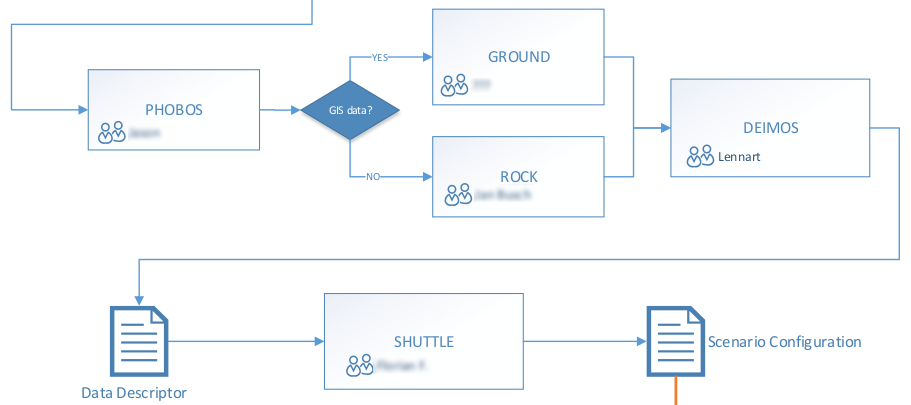
\includegraphics[height=114pt]{img/mars_websuite}\\
  \caption[]{Die Websuite des Mars Frameworks}
  \label{img:mars_websuite}
\end{figure}

\section{Geoinformationssystem (GIS)}
Geoinformationssysteme sind für die Erfassung, Bearbeitung, Organisation, Analyse und Präsentation von Geo-Daten zuständig. In der MARS Gruppe, welcher der Autor dieser Arbeit angehört Wird die Verwaltung des GIS durch MARS GROUND realisiert.\\
Im folgenden Abschnitt werden zwei Arten Rasterdaten zu klassifizieren beschrieben. Diese sind, die allgemeinen Rastertypen von GIS, sowie die speziellen der gängigsten GIS Anwendung, ArcGIS\footnote{\url{https://www.arcgis.com/}} unterteilt.

\subsection{Rasterdaten Typen}
Rasterdaten bestehen aus Ansammlungen von Bildpunkten (sog. Pixeln). Jeder Pixel hat einen Farbwert und eine Helligkeit. Aus diesen Pixeln setzen sich Bilder zusammen.\\
Bilder hoch zu skalieren ist somit mit Qualitätsverlust verbunden. Pixelbilder machen den Großteil aller digitalen Grafiken und Bilder aus. Im allgemeinen werden in GIS die folgenden Typen von Rasterdaten unterschieden\cite{mariuszMaster}.

\begin{itemize}
  \item Thematische Daten (Discrete data) stellen die Bodendaten oder Landnutzung dar.
  \item Kontinuierliche Daten (Continuous data) repräsentieren Ereignisse wie Bevölkerungszahlen oder Temperaturdaten, sowie spektrale Daten wie Luftaufnahmen oder Satellitenbilder.
  \item Bilder (Picture data) sind eingescannte Zeichnungen oder Karten, sowie Gebäudeaufnahmen.\\
\end{itemize}

\subsection{ArcGIS Rastertypen}
ArcGIS ist eine Anwendung zur Erstellung, Betrachtung und Bearbeitung von GIS Daten. Es zählt zu den besten Anwendungen, die es in diesem Bereich auf dem Markt gibt. In ArcGIS werden die folgenden vier Typen von Rasterdaten unterschieden.\\

\subsubsection{Raster als Grundkarten}\hspace*{\fill} \\
\label{sub:raster_grundkarte}Beim Raster als Grundkarte stellt ein oder mehrere gerasterte Bilder die Grundkarte dar. Darauf basierend können Informationen angezeigt werde. Diese Art von Karte ist der gängigste und in allen freien Kartendiensten, wie OpenStreetMap (OSM) oder Google Maps verfügbar. Häufig wird die Grundkarte zur Orientierung genutzt und mit weiteren Layern ergänzt. So können beispielsweise Fahrradwege als Vektor oder Oberflächenkarte über die Grundkarte gelegt werden.

\begin{figure}[H]
  \centering
  	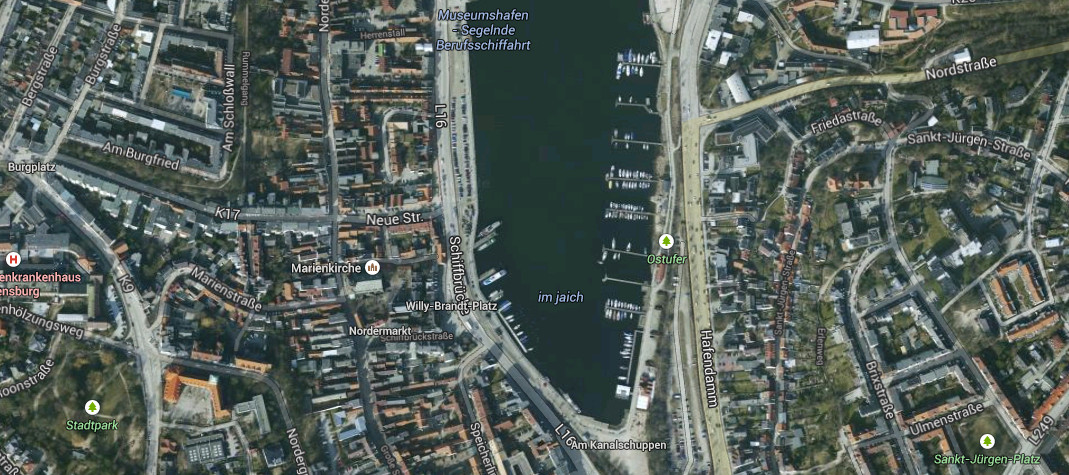
\includegraphics[height=114pt]{img/gis_Flensburg_raster}\\
  \caption[]{Luftaufnahme von Flensburg aus Google Maps}
  \label{img:gis_Flensburg_raster}
\end{figure}

\subsubsection{Raster als Oberflächenkarten}\hspace*{\fill} \\
Im Gegensatz zu dem Raster als Grundkarte liegt bei Oberflächenkarten die Fokussierung nicht auf infrastrukturellen Merkmalen. Vielmehr werden spatiale Daten durch bestimmte Farbgebung dargestellt. Somit geht es bei der Oberflächenkarte nicht um die reine Orientierung in einem Bereich, sondern vielmehr um die Darstellung gewonnener Ergebnisse. Diese können als Ergebnis einer GIS Operation entstehen. Häufige Anwendung sind Höhenkarten.

\begin{figure}[H]
  \centering
  	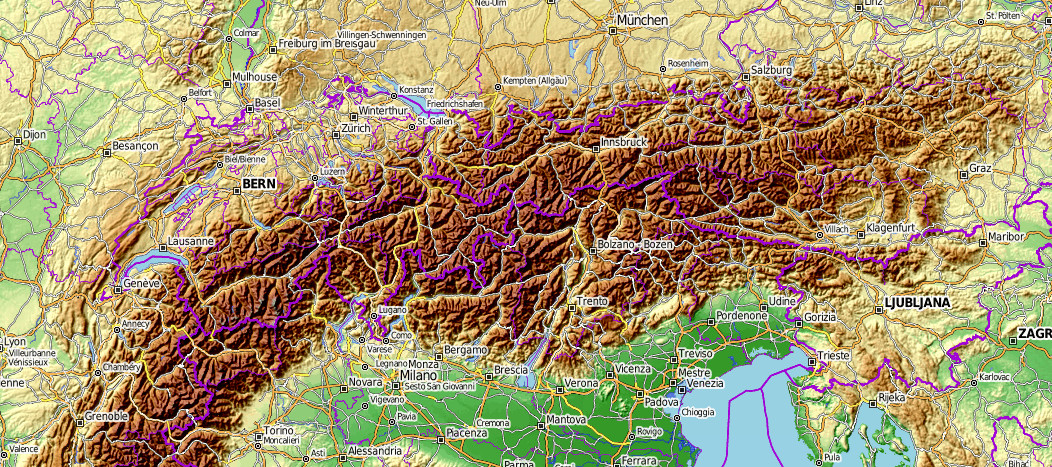
\includegraphics[height=114pt]{img/gis_alps}\\
  \caption[]{Höhenkarte der Alpen aus OpenStreetMap}
  \label{img:gis_alps}
\end{figure}

\subsubsection{Raster als thematische Karte}\hspace*{\fill} \\
Thematische Karten reduzieren die Anzahl der sichtbaren Merkmale auf ein Minimum. Somit bleiben lediglich die Form der Landfläche und entscheidende Merkmale, die für die Wiedererkennung notwendig sind übrig.\\
Die angezeigten Daten sind häufig stark schematisiert. Sie können Ergebnisse von GIS Operationen sein. Ein mögliches Anwendungsgebiet ist die Darstellung von Landnutzung. 

\begin{figure}[H]
  \centering
  	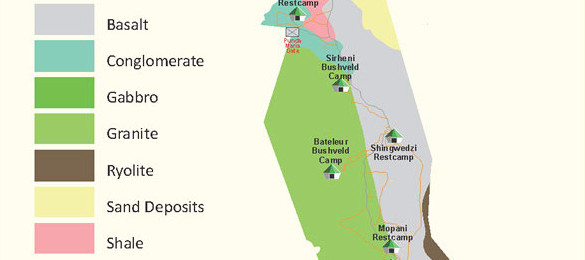
\includegraphics[height=114pt]{img/gis_thematisch}\\
  \caption[]{Thematische Darstellung des Krueger Nationalparks\footnotemark}
  \label{img:gis_thematisch}
\end{figure}
\footnotetext{\url{http://www.krugerpark.co.za/}}

\subsubsection{Raster als Beschreibung eines Objekts}\hspace*{\fill} \\
Hierbei werden Rasterbilder genutzt um ein Bereich einer Karte näher zu beschreiben. Dies wird z.B. verwendet, um Karten- oder Luftbilder an interessanten Stellen weiter anzureichern. 

\begin{figure}[H]
  \centering
  	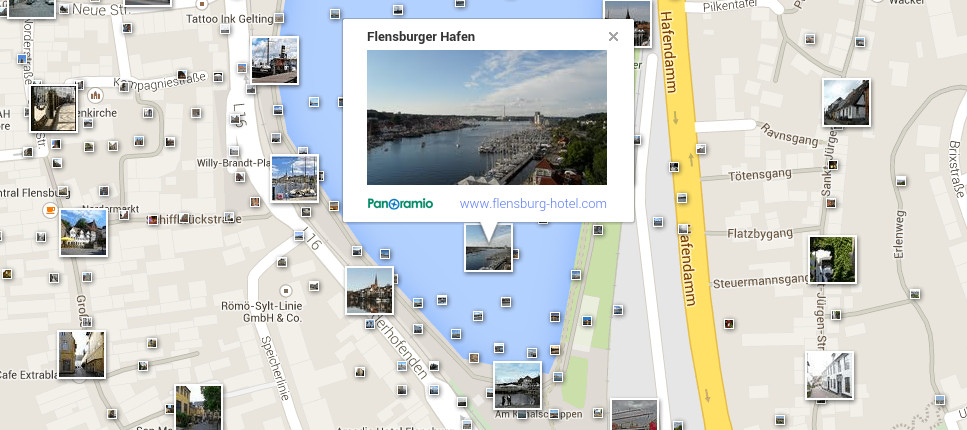
\includegraphics[height=114pt]{img/gis_beschreibung_object}\\
  \caption[]{Karte Flensburgs mit georeferenzierten Bildern aus Panoramio\footnotemark}
  \label{img:gis_beschreibung_object}
\end{figure}
\footnotetext{\url{http://www.panoramio.com/}}

\subsection{GIS Vektordaten}
Vektorgrafiken basieren im Gegensatz zu Rasterbildern auf mathematischen Formen. Hierzu zählen Kreise, Rechtecke und allgemeine Kurven. Ein Vektor hat immer ein Position bestehend aus X und Y. Die Art der Darstellung kann abhängig von dem gewünschten Einsatzgebiet unterschiedlich dargestellt werden. Dies macht sie erheblich flexibler, als Rasterdaten.\\
Vektorgrafiken eignen sich besonders für Schematische Darstellung und sind für Fotografien ungeeignet. Sie sind auf Grund ihrer Beschaffenheit beliebig skalierbar.\\
GIS Vektordaten bestehen aus Punkten, Linien und Polygonen.\vspace{.5em}

\subsubsection{Punkte}\hspace*{\fill} \\
Punkte sind das Grundelement, auf ihnen bauen die anderen Formen auf. Ein Punkt besteht aus einer X und einer Y Koordinate. Elemente, die als Punkt dargestellt werden sind z.B. Geopositionen.\vspace{.5em}

\subsubsection{Linien}\hspace*{\fill} \\
Linien werden durch eine mathematische Funktion dargestellt um die Form exakt zu beschreiben. Technisch wird eine Linie als zwei Punkte mit einer Verbindung umgesetzt.\vspace{.5em}

\subsubsection{Polygone}\hspace*{\fill} \\
Ein Polygon ist eine geschlossene Form bestehend aus Linien und Punkten. Es kann Eigenschaften, wie den Flächeninhalt besitzen. Beispiele für Polygone sind Rechtecke, Kreise und Dreiecke.


\section{Datawarehouse (DWH)}
Ein Data-Warehouse (DWH) ist eine Datenbank gestützte Anwendung, die Informationen zur Datenanalyse speichert. Dieser Ansatz findet zunehmend Verwendung für die Speicherung von geobezogenen Daten (siehe \cite{Kelling2009} \cite{McGuire2008} \cite{olap}).\par

In der Arbeit von Thiel-Clemen\cite{ThielClemen2013} aus dem Jahre 2013, wird beschrieben, wie sich zeitbezogene, spatiale Daten in einer relationalen Datenbank speichern lassen.\\
Hierzu wird für jede zu speichernde Dimension eine Datentabelle angelegt. Diese hängen von dem Domain spezifischen Use-Case ab. In Abbildung \ref{img:star_schema} wird die Bewegung von Geparden gemessen, sowie die Niederschlagsmenge an einem entsprechenden Messturm.

\begin{figure}[H]
  \centering
  	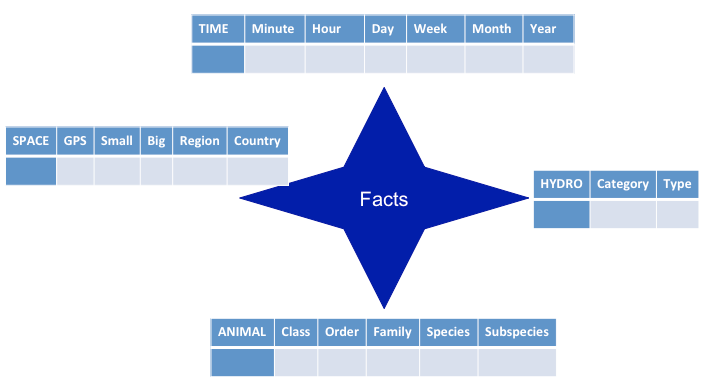
\includegraphics[width=\columnwidth]{img/star_schema}\\
  \caption[]{Sternansicht zur speicherung von Geodaten in einem DWH\cite{ThielClemen2013}}
  \label{img:star_schema}
\end{figure}


\section{Georeferenzierung}
Für die Verarbeitung von Geodaten ist es notwendig Daten aus GIS und DWH zu referenzieren. Hierbei führt die Art der Speicherung laut Baldowski\cite{mariuszMaster} im DWH zu einem Problem. Geodaten werden hierarchisch, zumeist in den Kategorien Länder, Kommunen, Städte und andere politische Grenzen gespeichert. Ländergrenzen ändern sich im Verlauf der Zeit und sind selbst zu einem gegebenen Zeitpunkt nicht immer eindeutig.\\
Beispielsweise zeigt die ukrainische Seite von Google Maps\footnote{\url{https://maps.google.com.ua/}} die Krim als Teil der Ukraine an, das russische Google Maps\footnote{\url{https://maps.google.ru/}} zeigt zwischen der Krim und der Ukraine eine Ländergrenze und in der deutschen und englischen Google Maps wird die Grenze als nicht feste Grenze (gestrichelt) dargestellt.\\
Hieraus ergibt sich die Problematik, dass Daten in Grenzgebieten nicht auf der Gleichen Hierarchieebene sein können, was für ökologische Daten nicht geeignet ist. Verstärkt wird dieses Problem, wenn Daten über einen längeren Zeitraum betrachtet werden sollen.\par

Eine Lösung für dieses Problem ist die Nutzung von Quad Trees\cite{quads}. Hierbei wird die Weltkarte in 4 Bereiche unterteilt. Jeder dieser Bereich besitzt 4 Teilbereiche. Diese besitzen wiederum Teilbereiche, bis zur gewünschten Detailstufe.\\
MARS ROCK nutzt die Implementation der Quad Trees, wie sie Microsoft bei Bing Maps einsetzt (siehe \cite{waldbiomasse}) wird. Hierbei erhalten die Bereiche eine Benennung, aus der die jeweilige Ebene hervorgeht. Es wird für jede weitere Detailstufe eine zusätzliche stelle hinzu genommen. Abbildung \ref{img:bing_quads} zeigt diese Struktur.

\begin{figure}[H]
  \centering
  	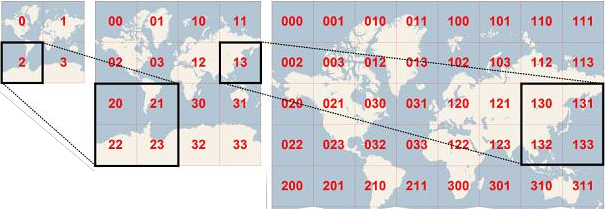
\includegraphics[width=\columnwidth]{img/bing_quads}\\
  \caption[]{Darstellung als Quads. Quelle: Bing Maps\cite{waldbiomasse}}
  \label{img:bing_quads}
\end{figure}

\subsection{Formate}
Um eine Georeferenzierung durchführen zu können ist es wichtig, dass die Daten in einer einheitlichen Form gespeichert werden.\\
Zuvor Müssen das Informationsmaterial in das Koordinatensystem eingepasst werden ein Ortsbezug hergestellt werden. Hierzu müssen Krümmungen der Erde angeglichen, oder beseitigt werden.\\
Baldowski Beschreibt in seiner Arbeit hierzu die folgenden Typen.

\subsubsection{GeoTIFF}\hspace*{\fill} \\
GeoTIFF (.geotiff) ist ebenso wie TIFF ein Format, welches verlustfrei speichert. GeoTIFF speichert zusätzlich zu den Rasterkarten die Geokoordinaten und den Bildausschnitt. Dieser Typ von Speicherung wird insbesondere für Satellitenaufnahmen verwendet.

\subsubsection{Erdas Imagine}\hspace*{\fill} \\
Bei diesem Format handelt es sich um ein Rasterformat, dass primär von kommerziellen Anwendungen verwendet wird. Die Dateiendung ist .img. Erdas Imagine wurde von ESRI\footnote{\url{http://www.esri.de/}} entwickelt.

\subsubsection{Shapefile}\hspace*{\fill} \\
Shapefiles (.shp) wurden ebenfalls von ESRI entwickelt. Dieses Format ist auf Grund seiner Einfachheit und geringen Overheads das gängigste zur Speicherung von GIS. In Shapefiles können jeweils nur eine Art von daten gespeichert werden (Punkte, Linien, Polygone).

\subsubsection{GeoJSON}\hspace*{\fill} \\
GeoJSON (.json, .geojson) sind Dateien, die Geoinformationen in JSON (JavaScript Object Notation) speichern. GeoJSON ist sehr einfach zu lesen und verfügt über eine geringe Dateigröße. Es wird sowohl in kommerziellen, als auch in freien Anwendungen verwendet.


\section{Verschneiden von Daten}
Für die Darstellung von Geodaten in einem bestimmten geographischem Gebiet ist es notwendig die Geodaten miteinander zu verschneiden. Hierbei werden die Ebenen skaliert und als Layer übereinander gelegt.

\subsection{Vektor und Vektor}
Bei der Verschneidung von Vektoren mit Vektoren muss zwischen den Vektortypen Punkt, Linie und Polygon unterschieden werden.

\subsubsection{Punkt in Polygon}\hspace*{\fill} \\
Bei der Verschneidung von Punkten im Polygon werden die Punkte, die sich innerhalb des Polygons befinden verschnitten.

\begin{figure}[H]
  \centering
  	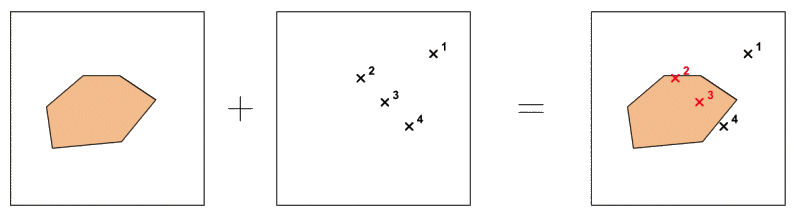
\includegraphics[width=\columnwidth]{img/punkt_in_polygon}\\
  \caption[]{Punkt in Polygon Verschnitt\cite{mariuszMaster}}
  \label{img:punkt_in_polygon}
\end{figure}

\subsubsection{Linie in Polygon}\hspace*{\fill} \\
Hierbei wird die Linie, die das Polygon durchläuft in zwei Teilsegmente geteilt.

\begin{figure}[H]
  \centering
  	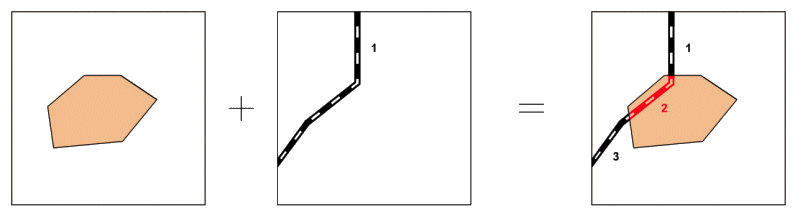
\includegraphics[width=\columnwidth]{img/linie_in_polygon}\\
  \caption[]{Linie in Polygon Verschnitt\cite{mariuszMaster}}
  \label{img:linie_in_polygon}
\end{figure}

\subsubsection{Polygon in Polygon}\hspace*{\fill} \\
Die Verschneidung von Polygonen mit Polygonen ergibt neue Formen als Summe der Teilmengen.

\begin{figure}[H]
  \centering
  	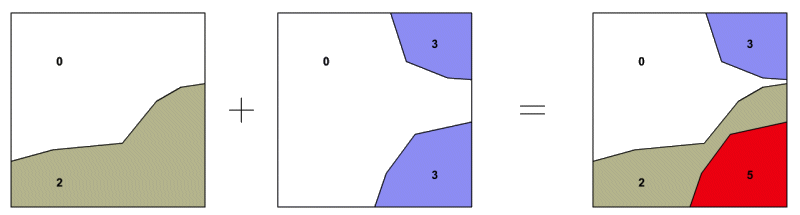
\includegraphics[width=\columnwidth]{img/polygon_in_polygon}\\
  \caption[]{Polygon in Polygon Verschnitt\cite{mariuszMaster}}
  \label{img:polygon_in_polygon}
\end{figure}

\subsection{Raster und Raster}
Für die Verschneidung von Rasterdaten untereinander ist es notwendig, dass die Datensätze verschiedene Voraussetzungen erfüllen.\\
Die Daten müssen den exakt gleichen Bereich referenzieren. Zudem muss die Qualität übereinstimmen. Dies muss pixelgenau durchgeführt werden.\\
Die eigentliche Verschneidung erfolgt durch eine pixelweise Differenzenbildung. Das Ergebnis enthält somit Die Summe an Informationen beider Bilder.

\subsection{Vektor und Raster}
Bei der Verschneidung von Vektor- und Rasterdaten werden die Vektordaten in die Form der Rasterdaten gebracht und dann wie Raster und Raster behandelt.


\section{Visualisierung}
Die Visualisierung von statischem Kartenmaterial ist seit der Entstehung von Google Maps, OSM und anderen Kartendiensten ein Bestandteil des Alltags geworden. Zunehmend wird die Darstellung von komplexeren spazialen Daten für die Forschung interessant (siehe \cite{gps_collars} \cite{wms_flow_mapping}).\\
Für die Darstellung von Daten mit speziellen Anforderungen gibt es unterschiedliche Anwendungsfälle. Diese erfordern entsprechende Lösungen.

\subsection{Bewegungsdaten}
Der Bereich der Bewegungsdaten ist insbesonders in der Erforschung von Tierbewegungen von großer Bedeutung\cite{gps_collars}.\\
Durch die fortgeschrittene technische Entwicklung sind GPS Sensoren mittlerweile klein und kostengünstig geworden. Hierdurch ist es möglich Tiere mit Peilsensoren zu versehen und Bewegungsprofile zu erstellen.\\
Die Bereitstellung solcher Daten im Web ermöglicht einen weltweiten Austausch zwischen Forschergruppen und verbessert die Vergleichbarkeit und Qualität der Auswertungen erheblich.\\
Movebank\footnote{\url{https://www.movebank.org/}} ist ein derartiges Projekt. Es bietet frei zugängliche Bewegungsdaten von Tieren. In Abbildung \ref{img:movebank} wird die Bewegung von Weißstörchen dargestellt.

\begin{figure}[H]
  \centering
  	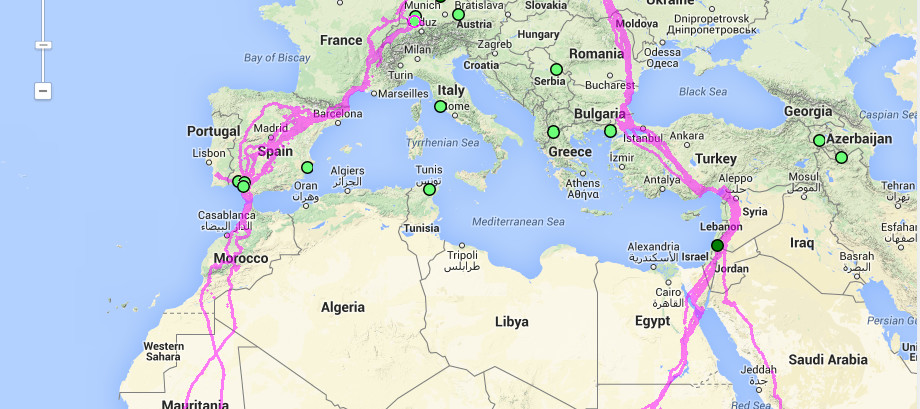
\includegraphics[height=114pt]{img/movebank}\\
  \caption[]{Movebank Vogelbewegung}
  \label{img:movebank}
\end{figure}


\subsection{Zeitbezogene Daten}
\label{sub:zeitbezogene_daten}
Für die Erforschung, der Auswirkung des Klimawandels ist es wichtig Aufnahmen von gewissen Flächenabschnitten zu vergleichen. In der Vergangenheit mussten diese Messungen anhand von Markierungen, Boden oder Luftbildern gemacht werden. Dank fortgeschrittener Satellitentechnik sind großflächige Aufnahmen möglich geworden.\par

Zu diesem Zweck hat die australische Regierung den Australian Geoscience Data Cube (AGDC) entwickelt. Dieser erlaubt die umfangreiche Auswertung von Satellitenmaterial. So wird mit Hilfe von Satelliten mit spezieller Kameras Wasserbestände in Australien gemessen.\\
Dieses Bildmaterial von unterschiedlichen Satelliten wird geclustert und zu einer Karte zusammengefügt. Dieser Vorgang wird regelmäßig wiederholt. Aus den Differenzen der Karten wird eine Heatmap gebildet, die anzeigt, wie oft ein bestimmter Bereich überflutet wurde. Diese Heatmap ist auf der Seite der australischen Regierung offen einzusehen (siehe Abbildung \ref{img:agcd_flood}).

\begin{figure}[H]
  \centering
  	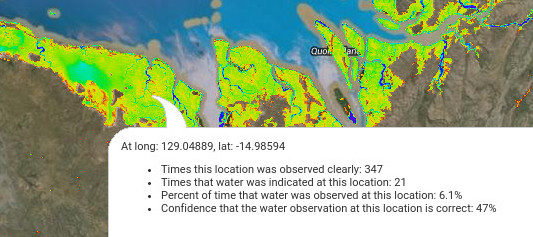
\includegraphics[height=114pt]{img/agcd_flood}\\
  \caption[]{Überschwemmungskarte Australien. Quelle: AGDC\footnotemark}
  \label{img:agcd_flood}
\end{figure}
\footnotetext{\url{http://www.ga.gov.au/flood-study-web/#/water-observations}}


\section{vergleichbare Systeme}
Es existieren bereits komplette Systeme, zur Visualisierung von zeitbezogenen spazialen Daten. Diese haben entsprechend ihrem Anwendungsgebiet unterschiedliche Architekturen.

\subsection{Australian Geoscience Data Cube (AGDC)}
Australiens Data Cube, der bereits in Abschnitt \ref{sub:zeitbezogene_daten} erwähnt wurde, gehört zu den größten derartigen Installationen weltweit. Das Team besteht aus 673 Mitarbeitern und hat bis zum Juli 2014 wurden 4PB, also über 4.000TB Daten gesammelt\cite{agdc}. Mit 160TB Arbeitsspeicher und 57.472 Kernen belegt der AGDC Platz 32 der Liste von Supercomputern\footnote{\url{http://top500.org/}}.\\
Zur Speicherung von Daten wird PostgreSQL mit der Erweiterung POSTGIS für GIS Daten eingesetzt. Als Programmiersprache wird Python eingesetzt und der Quellcode ist seit Juni 2014 auf GitHub verfügbar.\par

Der AGDC ist eine Lösung, dessen Einsatzmöglichkeiten auf keinen einzelnen Einsatzfall beschränkt sind. Stattdessen werden eine Vielzahl von Projekten umgesetzt. Die beiden populärsten Projekte sind die bereits erwähnte Darstellung von Hochwasserbereichen und einer Visualisierung von Vegetationsentwicklung\cite{agdc2}.

\subsection{WMS flow mapping Services}
\label{sub:flow_mapping}
In der Arbeit  von Guo et al.\cite{wms_flow_mapping} wird das \enquote{Web Map Service} (WMS) Protokoll des \enquote{Open Geospatial Consortium} (OGC) um die effiziente Erstellung von Strömen erweitert. Dies dient der Verbesserung, der Analyse von Echtzeit Daten, insbesondere aus sozialen Medien.\\
WMS ist ein Standard Protokoll, das mit einer einfachen HTTP Schnittstelle arbeitet. Es wird von allen gängigen GIS Anwendungen unterstützt, hierzu zählen die im MARS Framework verwendeten ArcGIS und der GeoServer.\par

Web Flow Map Services (WFMS) ermöglicht eine effiziente Generierung von Strömen. Dies ist insbesondere dann wichtig, wenn ein Diagramm auf Basis von großen Datenmengen erstellt werden soll. Ein Beispiel für ein Flow Chart mit großen Datenmengen ist das Umzugsverhalten eines ganzen Landes über mehrere Jahre hinweg betrachtet. Die Komplexität verbessert sich durch den Flow Algorithmus in WFMS von $O(n^2 )$ auf $O(n \log (n))$.\par

Der Versuchsaufbau des WFMS Frameworks entspricht Abbildung \ref{img:wfms}. Die Dateneingaben der Echtzeitdaten und Daten aus dem Modell werden im Rechenzentrum parallel berechnet, falls sie im Cache nicht vorhanden sind. Hieraus Entstehen Zwischenergebnisse, die über WFMS an das Frontend übertragen werden.\\
Die JavaScript Bibliothek OpenLayers stellt ein \enquote{Raster als Grundkarte} dar (siehe Abschnitt \ref{sub:raster_grundkarte}). Mögliche Datenquellen der Karten sind Google Maps, OSM und der GeoServer. Auf dieser Karte wird die Flow Karte dargestellt. Zu beachten ist, dass es sich bei dem Ergebnis des Servers nicht um eine Vektorkarte, sondern um ein gerastertes Bild handelt. OpenLayers muss diese skalieren und der Grundkarte als Layer hinzufügen.

\begin{figure}[H]
  \centering
  	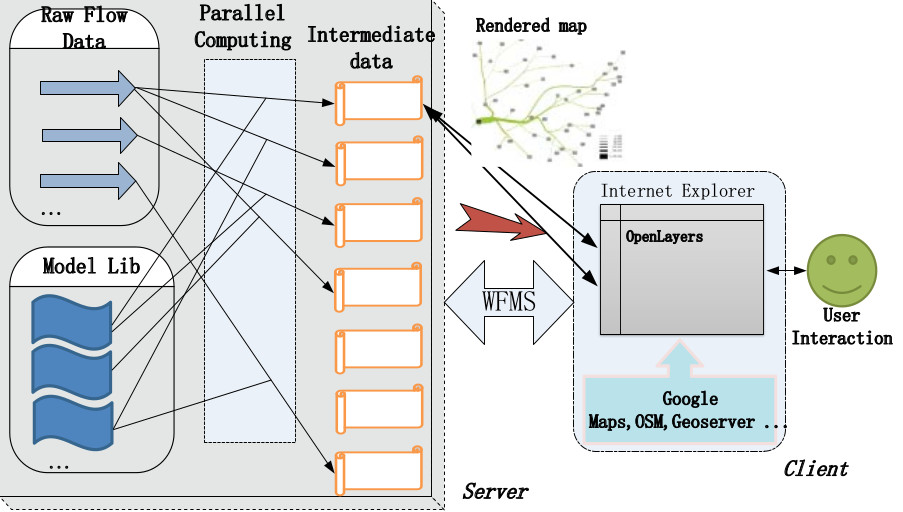
\includegraphics[width=\columnwidth]{img/wfms}\\
  \caption[]{WFMS Framework\cite{wms_flow_mapping}}
  \label{img:wfms}
\end{figure}

\section{DEIMOS}
Das Ziel für das Grundprojekt ist es, die wissenschaftliche Grundlage für DEIMOS zu entwickeln und einen ersten \enquote{Durchstich} umzusetzen. Hierzu soll das Frontend inklusive Darstellung der Daten aus ROCK und GROUND in Tabellenansicht, als minimal Anforderung implementiert werden.\\

\subsection{MEAN-Stack}
Der Softwarestack für DEIMOS ist rein JavaScript basiert und ist für die drei Komponenten der der Websuite (siehe Abbildung \ref{img:mars_websuite}) größtenteils identisch. Lediglich das SHUTTLE wird Teile in C\# enthalten. \\
Das Akronym \enquote{MEAN} besteht aus den drei Anfangsbuchstaben der enthaltenen Frameworks. Der JavaScript MEAN-Stack besteht aus folgenden Komponenten:

\subsubsection{MongoDB}\hspace*{\fill} \\
MongoDB ist ein Dokumenten basiertes Datenbanksystem, dass seine Daten nicht in relationalen Tabellen abspeichert. Stattdessen wird in binären JSON Dateien gespeichert, sog. BSON Dateien. MongoDB ist die Standard Datenbank im MEAN-Stack und zudem sehr einfach zu bedienen. Aus diesem Grund ist sie derzeit für die Speicherung von Metadaten der zu importierenden Daten durch PHOBOS angedacht.\\
In den vergangenen Wochen kam jedoch die Frage auf, inwiefern die Nutzung dieser Speicherungsform geeignet sei. MongoDB ist besonders gut für die Speicherung von Objekten geeignet. Die zu speichernden Daten werden jedoch auf viele unterschiedliche Arten abgefragt.\\
Wenn angenommen wird, dass Messdaten nach Projekten und Tierarten gespeichert sind würde eine Suche in einem geografischen Bereich eine Vielzahl von Objekten betreffen aus denen jeweils Teilmengen benötigt wird.\\
Da nicht vorausgesagt werden kann, wie die Form der Abfrage am ende aussehen wird und MongoDB keine Querreferenzierung unterstützt gilt die Frage zu klären, welche Alternativen in Frage kommen.\par

Realistisch kommen zwei Datenbanktypen in Frage. Zum einen ist die Nutzung einer relationalen Datenbank sehr üblich. In der Literatur wird PostgreSQL mit der Erweiterung POSTGIS mehrfach erwähnt (siehe \cite{wms_flow_mapping} \cite{waldbiomasse}). Eine MariaDB Datenbank kommt als Alternative in Frage.\\
Auf Grund der starken Abhängigkeiten der Messdaten zueinander ist die Nutzung einer Graphdatenbank ebenfalls eine Möglichkeit. Solche Datenbanken Bilden ihre Daten auf Knoten und Kanten ab. Hierbei können sowohl Knoten, als auf Kanten mit Eigenschaften versehen sein.\\
Im Grundprojekt gilt es das Problem der Datenbankwahl tiefer zu durchdringen und dann eine Entscheidung zu treffen.\vspace{.5em}

\subsubsection{ExpressJS}\hspace*{\fill} \\
Express ist ein Web Framework für NodeJS, das zudem die Erstellung von REST APIs unterstützt.\vspace{.5em}

\subsubsection{AngularJS}\hspace*{\fill} \\
Angular ist ein Web Framework für JavaScript. Es erweitert die HTML Syntax für die Nutzung von dynamischen Inhalten. Das von Google entwickelte Framework nutzt Model-View-Controller (MVC) zur Handhabung und Aktuallisierung von Daten. Angular spricht über xmlHttpRequests mit der ExpressJS API.\vspace{.5em}

\subsubsection{NodeJS}\hspace*{\fill} \\
Node ist eine Laufzeit Umgebung, die es ermöglicht JavaScript serverseitig auszuführen. Node läuft auf Basis der JavaScript V8 Engine, die von Google für den Chrome Browser entwickelt wurde. Es läuft in einem einzigen Thread und verfügt über eine \enquote{non-blocking I/O API}. Diese führt dazu, dass der Thread niemals angehalten werden muss. Stattdessen werden Berechnungen mit einem Callback versehen, der den Programmablauf beeinflusst.

\subsection{Kartendarstellung}
Die Kartendarstellung im Browser soll nach aktueller Planung LeafletJS\footnote{\url{http://leafletjs.com/}} übernehmen. Leaflet gehört mit ObenLayers zu den bekanntesten, frei verfügbaren JavaScript Bibliotheken zur Kartendarstellung.\\
Die Recherche dieser Arbeit hat ergeben, dass in komplexeren Einsatzgebieten OpenLayers bevorzugt wird (siehe \cite{mariuszMaster} \cite{quads} \cite{wms_flow_mapping}).\\
OpenLayers ist jedoch mit 770kb Dateigröße ein sehr schwergewichtiges JavaScript Framework, Leaflet hingegen umfasst lediglich 125kb. JQuery, dass im allgemeinen als nicht sonderlich leichtgewichtig gilt ist lediglich 84kb groß.\\
Diese Größen mögen sich auf den ersten Blick als nicht relevant erweisen. Hierbei wird jedoch vernachlässigt, dass diese Frameworks beim Seitenaufbau geladen werden müssen, was insbesonders bei langsamen Internetverbindungen zur Beeinträchtigung der Benutzbarkeit führt.\\
Zudem ist Leaflet ein jüngeres und leichter bedienbares Framework. Es wird deshalb zunächst als bevorzugtes betrachtet. Sollte sich herausstellen, dass eine Umsetzung hiermit zu schwierig oder nicht möglich ist, wird eine Umstellung durchgeführt.


\section{Zusammenfassung}
In dieser Arbeit wurden die Grundlagen der Arbeit von DEIMOS beschrieben. Es wurden zudem Technologieentscheidungen diskutiert. Einige dieser Entscheidungen können sich jedoch in der Zukunft ändern.\\
DEIMOS wird nach seiner Fertigstellung für die Visualisierung von Simulationsdaten zuständig sein und eine Auswahl von Daten zur Erstellung einer Simulation an das SHUTTLE übergeben können. Für das Grundprojekt soll eine erste Vorabversion erstellt werden.

\bibliographystyle{IEEEtran}
\bibliography{bibtemplate_samples}


\end{document}